В прошлом семестре была начата разработка веб-сайта, представляющего программный комплекс COEX интернету. Была создана главная страница и небольшое наполнение контентом. На данный семестр были поставлены следующие задачи:

\begin{itemize}
  \item исправление дизайна;
  \item добавление вывода новостей;
  \item актуализация информации, представленной на сайте.
\end{itemize}

\subsubsection{Исправление дизайна и актуализация информации}

Для новых плагинов созданы иконки (рис.~\ref{lob_1:lob_1}).

\begin{figure}[h!]
\center{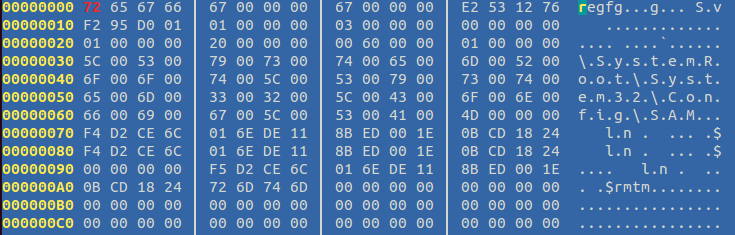
\includegraphics[width=0.8\linewidth]{lob_1}}
\caption{Иконки модулей}
\label{lob_1:lob_1}
\end{figure}

Общая архитектурная схема системы из изображения была свёрстана в HTML + CSS код (рис.~\ref{lob_2:lob_2} и~\ref{lob_3:lob_3}).

\begin{figure}[h!]
\center{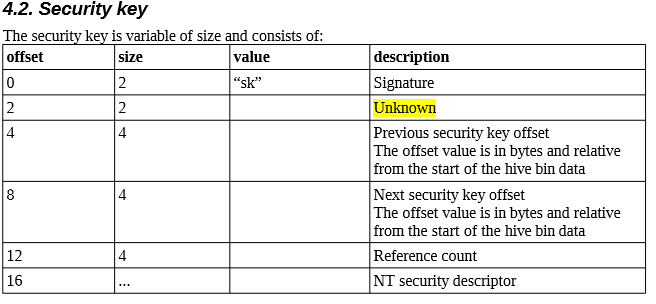
\includegraphics[width=1\linewidth]{lob_2}}
\caption{HTML + CSS код блока схемы системы}
\label{lob_2:lob_2}
\end{figure}

\begin{figure}[h!]
\center{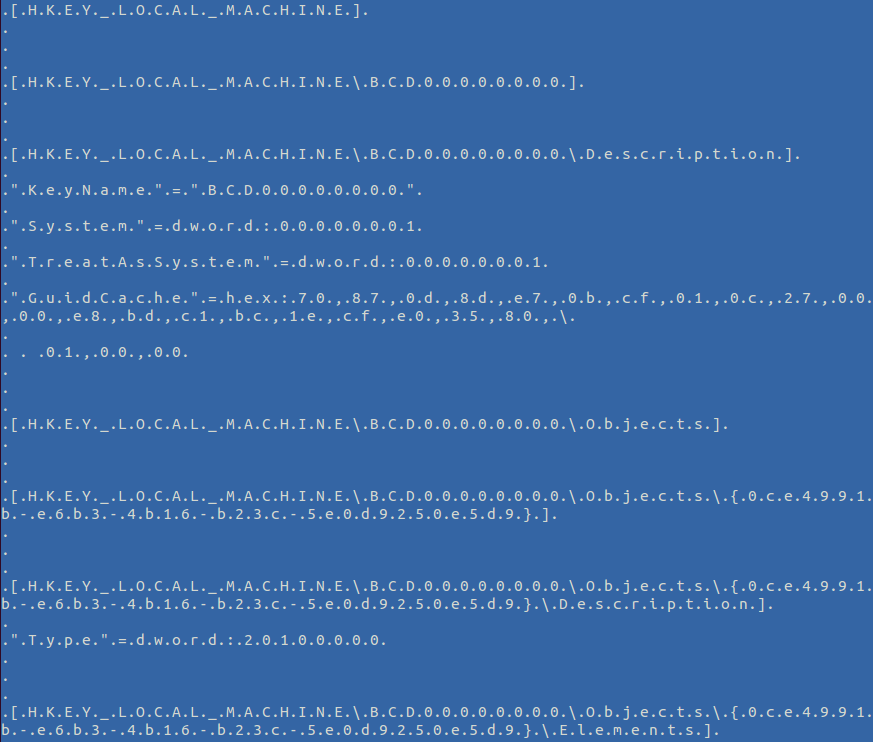
\includegraphics[width=1\linewidth]{lob_3}}
\caption{Схема системы}
\label{lob_3:lob_3}
\end{figure}

Доработана нижняя часть сайта (футер), представленный на рисунке~\ref{lob_4:lob_4}.

\begin{figure}[h!]
\center{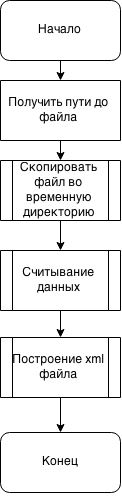
\includegraphics[width=1\linewidth]{lob_4}}
\caption{Футер сайта}
\label{lob_4:lob_4}
\end{figure}

\subsubsection{Добавление вывода новостей}

Создана группа в социальной сети Вконтакте, где в дальнейшем будут выкладывать новости проекта (рис.~\ref{lob_5:lob_5}).

\begin{figure}[h!]
\center{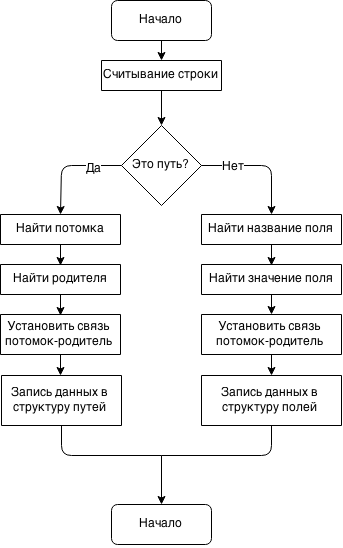
\includegraphics[width=1\linewidth]{lob_5}}
\caption{Группа проекта в ВК}
\label{lob_5:lob_5}
\end{figure}

Используя API, предоставляемый социальной сетью Вконтакте, был сгенерирован виджет новостей проекта для сайта (рис.~\ref{lob_6:lob_6} и~\ref{lob_7:lob_7}).

\begin{figure}[h!]
\center{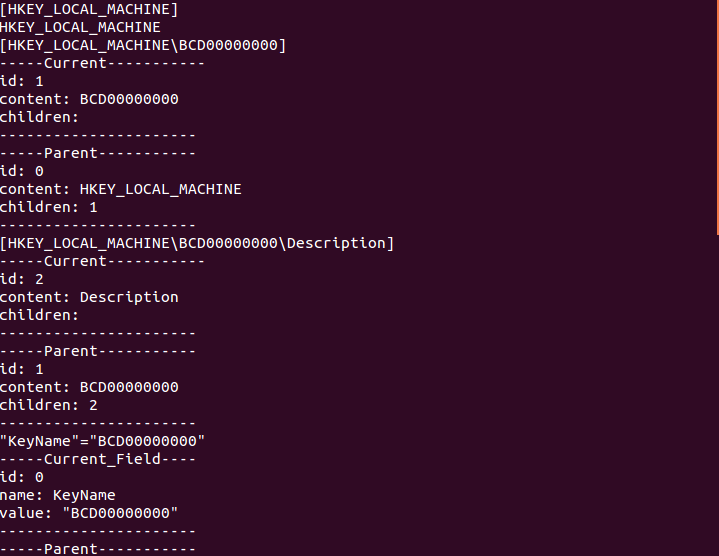
\includegraphics[width=0.7\linewidth]{lob_6}}
\caption{Код виджета}
\label{lob_6:lob_6}
\end{figure}

\begin{figure}[h!]
\center{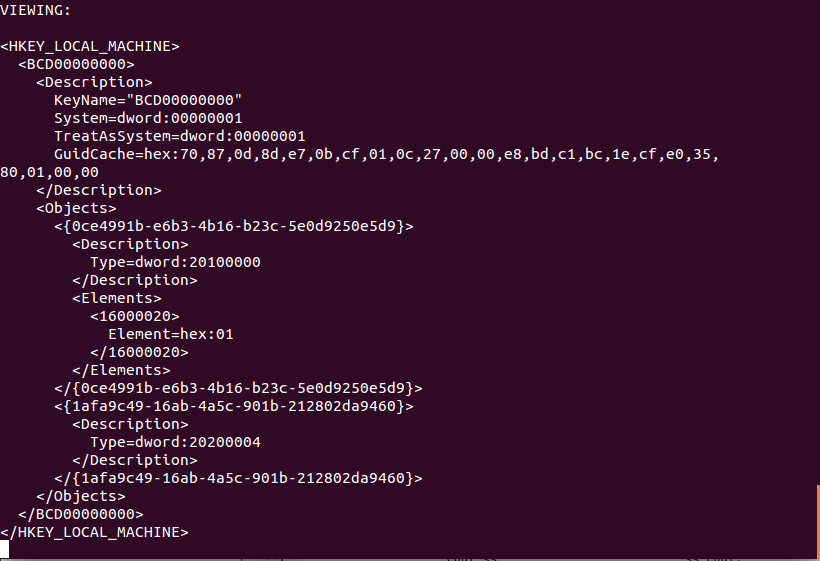
\includegraphics[width=1\linewidth]{lob_7}}
\caption{Новости на сайте}
\label{lob_7:lob_7}
\end{figure}

\clearpage
	
